% \newcommand{\xqq}{x862}

\todo[inline]{relire}
Nous nous intéressons en premier lieu aux programmes malveillants fonctionnant sur des ordinateurs personnels et en particulier les programmes compilés, qui s'exécutent nativement dans le langage assembleur spécifique au processeur de la machine.

\ijym{Mieux délimiter les figures}

\section{Compilation et fichiers exécutables}
Un exécutable est en général d'abord écrit dans un langage de haut niveau. Chacun de ses modules est ensuite compilé en un fichier objet (binaire) encodant le langage assembleur spécifique à la machine. La dernière étape est l'édition de liens qui consiste à regrouper tous les fichiers objets en un exécutable unique.

Prenons l'exemple d'un simple \helloworld\ en C (Figure \ref{fig:helloword_c}). Il est uniquement composé d'un appel à la fonction \texttt{printf} permettant l'affichage, à l'exécution, de la chaîne de caractère ``Hello, world.''.
Une implémentation possible en assembleur \nasm\ \xq\ pouvant tourner sous une distribution GNU/Linux est donnée en figure \ref{fig:helloword_asm}. Il est alors composé de deux appels système vers le noyau Linux : une première (sys$\_$write) permettant l'affichage de la chaîne et une seconde (sys$\_$exit) permettant de fermer le processus.
On peut déjà remarquer que le programme est séparé en une section de données (\pdata) contenant la chaîne de caractère à afficher et une section de code (\ptext) contenant le code assembleur à exécuter.
\begin{figure}
\begin{lstlisting}[language={C}]
int main(int argc, char* argv[]){
  printf("Hello, world.");
}
\end{lstlisting}
\caption{Code C de \helloworld}
\label{fig:helloword_c}
\end{figure}


\begin{figure}
\begin{lstlisting}[language={[x86masm]Assembler}, escapechar=~]
section .data
msg     db      "Hello, world", 0xa	; ~La chaîne à afficher~
len     equ     13                      ; ~La taille de la chaîne~

section .text
global _start

_start:
; ~Afficher la chaîne de caractères~
mov     eax, 4      ; ~Numéro d'appel système (sys$\_$write)~
mov     ebx, 1      ; ~Premier argument : le fichier de sortie (ici stdout)~
mov     ecx, msg    ; ~Second argument : un pointeur vers la châine à afficher~
mov	edx, len    ; ~Troisième argument : la taille de la chaîne~
int     0x80        ; ~Appel effectif au noyau~

; ~Fermer proprement le programme~
mov     eax, 1      ; ~Numéro d'appel système (sys$\_$exit)~
mov	ebx, 0	    ; ~Premier argument : le code de retour (0 : normal)~
int     0x80	    ; ~Appel au noyau~
\end{lstlisting}
\caption{Code assembleur \xq\ de \helloworld}
\label{fig:helloword_asm}
\end{figure}

Le fichier binaire exécutable résultant de la compilation est un exécutable binaire pour Linux, sous format ELF.
% Le format ELF est structuré de la manière suivante. 
Comme indiqué sur la figure \ref{fig:structure_elf}, il contient des entêtes dans lesquels sont indiqués des informations générales sur le binaire telle que le point d'entrée du programme, les différentes sections du programme (leur taille, leurs adresses) et les différentes sections : ici une section \pdata\ (Figure \ref{fig:data_helloworld}) contient les données du programmes (dont la chaîne de caractères ``Hello World'') et une section \ptext\ (Figure \ref{fig:text_helloworld}) contenant le code assembleur à exécuter.
À l'instar de la figure \ref{fig:structure_elf} donnant une structure simplifiée du format ELF pour Linux, la figure \ref{fig:structure_pe} donne un aperçu du format des fichiers exécutables pour un binaire \xq\ sous Windows (format PE).

\begin{figure}
\begin{center}
\subfigure[Fichier ELF]{
\begin{tabular}[b]{|c|}
\hline
Entête ELF\\
\hline
Table des entêtes du programme\\
\hline
Section .text\\
\hline
Section .rodata\\
\hline
Section ...\\
\hline
Section .data\\
\hline
Table des sections\\
\hline
\end{tabular}
\label{fig:structure_elf}
}
\subfigure[Fichier PE]{
\begin{tabular}[b]{|c|}
\hline
Entête PE\\
\hline
Table des sections\\
\hline
Sections de code\\
\hline
Sections d'imports\\
\hline
Sections de données\\
\hline
\end{tabular}
\label{fig:structure_pe}
}
\ijym{à expliquer / détailler}
\end{center}
\caption{Format des exécutables ELF (Linux) et PE (Windows)}
\label{fig:structure_exe}
\end{figure}

\begin{figure}
\begin{center}
\begin{tabular}{|c|c|l|l|}
\hline
Emplacement dans le fichier & Adresses de chargement & Octets & Caractères ascii\\ 
\hline
94 & 80490a4 & 48 65 6c 6c 6f 2c 20 & H e l l o ,   \\
9b & 80490ab & 77 6f 72 6x 64 & W o r l d \\
a0 & 80490b0 & 0a & Fin de chaîne       \\
\hline
\end{tabular}
\end{center}
\caption{Section \pdata\ de \helloworld}
\label{fig:data_helloworld}
\end{figure}

\begin{figure}
\begin{center}
\begin{tabular}{|c|c|l|l|}
\hline
Emplacement dans le fichier & Adresses de chargement & Octets & Instruction\\ 
\hline
80 & 8048080 & b8 04 00 00 00 & mov    eax,0x4       \\
85 & 8048085 & bb 01 00 00 00 & mov    ebx,0x1       \\
8a & 804808a & b9 a4 90 04 08 & mov    ecx,0x80490a4 \\
8f & 804808f & ba 11 00 00 00 & mov    edx,0x11      \\
94 & 8048094 & cd 80          & int    0x80          \\
96 & 8048096 & bb 00 00 00 00 & mov    ebx,0x0       \\
9b & 804809b & b8 01 00 00 00 & mov    eax,0x1       \\
a0 & 80480a0 & cd 80          & int    0x80          \\
\hline
\end{tabular}
\end{center}
\caption{Section \ptext\ de \helloworld}
\label{fig:text_helloworld}
\end{figure}


% \x64
\paragraph{Analyse de binaires}
La principale difficulté lors de l'analyse d'un programme malveillant est que le code source n'est pas disponible à l'analyste qui doit se contenter du fichier binaire compilé.
Un programme compilé se présente donc sous la forme d'un fichier binaire contenant le code machine devant être lancé à l'exécution du programme ainsi que des informations de chargement du binaire : la distinction de différentes sections, les adresses mémoires auxquelles le système devra les charger en mémoire ainsi que les librairies du système dont il a besoin et qui devront être chargées.

La principale tâche de l'analyste est alors d'extraire du fichier binaires les informations utiles et surtout d'analyser les parties de code assembleur de l'exécutable. Nous détaillerons, dans la suite de ce chapitre, des spécificités du langage assembleur considéré, les difficultés rencontrées par l'analyste et certaines techniques de protection.

\label{section:assembleur}
\section{Assembleur \xq\ et \xs}
L'architecture la plus fréquente sur les ordinateurs personnels est celle des processeurs Intel CISC avec le jeu d'instructions \xq\ pour les machines adressant la mémoire sur 32 bits, et le jeu d'instructions \xs\ pour celles adressant la mémoire sur 64 bits.
\todo[inline]{
Différence 32 / 64 bits ?
}

\paragraph{Architecture de Harvard modifiée.}
Les ordinateurs actuels fonctionnent selon une version modifiée de l'architecture de Harvard \cite{ibm_mark1} \todo{citation sur mod harvard arch ou on repasse à Neumann ?}\jym{Harvard ou Von Neumann ?}.
La première implémentation de l'architecture de Harvard était L’ASCC (Automatic Sequence Controlled Calculator) d'IBM, également appelé le Mark I et considérée comme le premier calculateur universel, en 1944 . 
Il lisait les instructions sur des cartes perforées et les données étaient entrées manuellement à l'aide d'interrupteurs. 
Ainsi le code exécutable était physiquement non modifiable et séparé des données. 


L'architecture de Von Neumann, qui acceptait la modification de la logique des programmes, était limitée à l'utilisation d'un seul bus de données entre le processeur et la mémoire.
Cette restriction limite grandement les capacités de lecture et écriture mémoire d'une machine utilisant le modèle de Von Neumann. On appelle alors architecture de Harvard modifiée l'architecture de Harvard à plusieurs bus mémoire dans laquelle les instructions et les données sont stockées dans la même mémoire et donc accessibles autant en lecture qu'en écriture.

Dans ce modèle la machine est articulée autour du processeur et de son unité de contrôle chargée de synchroniser les autres composants, d'exécuter les instructions du binaire chargé en mémoire, de gérer les entrées et les sorties, de lire et d'écrire dans la mémoire et les registres. L'unité arithmétique et logique opère toute l'arithmétique du processeur et modifie les drapeaux du registre d'état en conséquence selon les résultats des opérations effectuées. Par exemple si une addition provoque un débordement d'entier, c'est à dire que le résultat de l'addition ne peut être stocké dans un seul registre, alors le drapeau OF (overflow) est passé à 1.
Une organisation simplifiée d'une machine utilisant le modèle de Harvard modifié est donnée Figure \ref{fig:arch_harvard_mod}.

\begin{figure}
\begin{center}
% Graphic for TeX using PGF
% Title: /home/aurelien/these/supports/architecture/arch.dia
% Creator: Dia v0.97.2
% CreationDate: Wed Jun 18 11:06:57 2014
% For: aurelien
% \usepackage{tikz}
% The following commands are not supported in PSTricks at present
% We define them conditionally, so when they are implemented,
% this pgf file will use them.
\ifx\du\undefined
  \newlength{\du}
\fi
\setlength{\du}{15\unitlength}
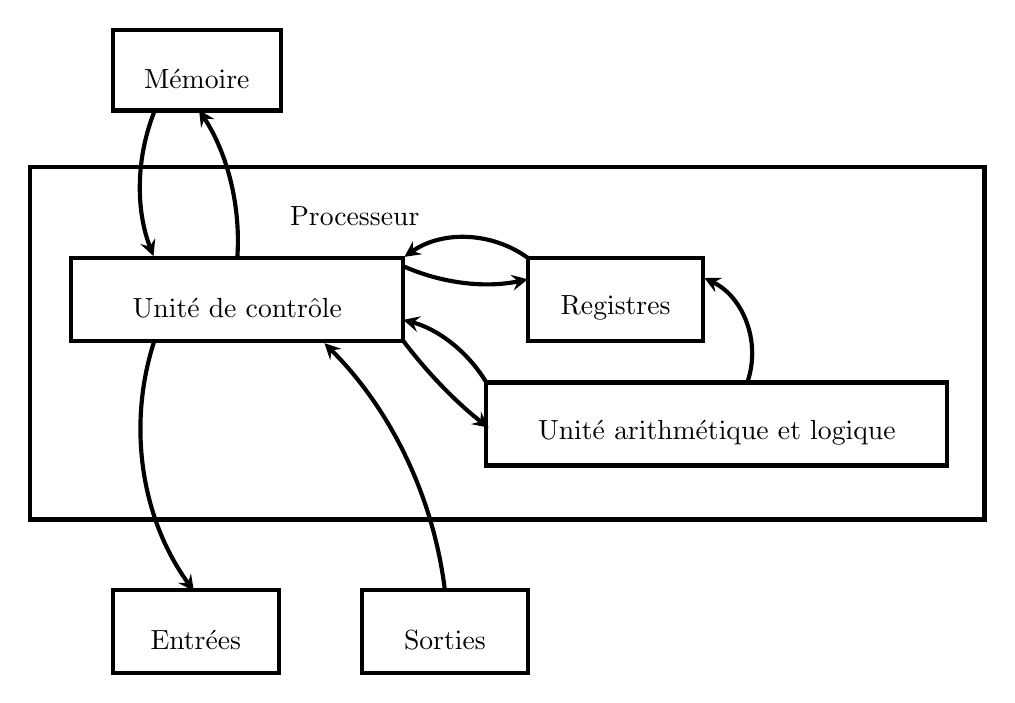
\begin{tikzpicture}
\pgftransformxscale{1.000000}
\pgftransformyscale{-1.000000}
\definecolor{dialinecolor}{rgb}{0.000000, 0.000000, 0.000000}
\pgfsetstrokecolor{dialinecolor}
\definecolor{dialinecolor}{rgb}{1.000000, 1.000000, 1.000000}
\pgfsetfillcolor{dialinecolor}
\definecolor{dialinecolor}{rgb}{1.000000, 1.000000, 1.000000}
\pgfsetfillcolor{dialinecolor}
\fill (16.000000\du,5.800000\du)--(16.000000\du,14.300000\du)--(39.000000\du,14.300000\du)--(39.000000\du,5.800000\du)--cycle;
\pgfsetlinewidth{0.100000\du}
\pgfsetdash{}{0pt}
\pgfsetdash{}{0pt}
\pgfsetmiterjoin
\definecolor{dialinecolor}{rgb}{0.000000, 0.000000, 0.000000}
\pgfsetstrokecolor{dialinecolor}
\draw (16.000000\du,5.800000\du)--(16.000000\du,14.300000\du)--(39.000000\du,14.300000\du)--(39.000000\du,5.800000\du)--cycle;
% setfont left to latex
\definecolor{dialinecolor}{rgb}{0.000000, 0.000000, 0.000000}
\pgfsetstrokecolor{dialinecolor}
\node[anchor=west] at (16.450000\du,10.245000\du){};
% setfont left to latex
\definecolor{dialinecolor}{rgb}{0.000000, 0.000000, 0.000000}
\pgfsetstrokecolor{dialinecolor}
\node[anchor=west] at (22.000000\du,7.000000\du){Processeur};
\definecolor{dialinecolor}{rgb}{1.000000, 1.000000, 1.000000}
\pgfsetfillcolor{dialinecolor}
\fill (17.000000\du,8.000000\du)--(17.000000\du,10.000000\du)--(25.000000\du,10.000000\du)--(25.000000\du,8.000000\du)--cycle;
\pgfsetlinewidth{0.100000\du}
\pgfsetdash{}{0pt}
\pgfsetdash{}{0pt}
\pgfsetmiterjoin
\definecolor{dialinecolor}{rgb}{0.000000, 0.000000, 0.000000}
\pgfsetstrokecolor{dialinecolor}
\draw (17.000000\du,8.000000\du)--(17.000000\du,10.000000\du)--(25.000000\du,10.000000\du)--(25.000000\du,8.000000\du)--cycle;
% setfont left to latex
\definecolor{dialinecolor}{rgb}{0.000000, 0.000000, 0.000000}
\pgfsetstrokecolor{dialinecolor}
\node at (21.000000\du,9.206667\du){Unité de contrôle};
\definecolor{dialinecolor}{rgb}{1.000000, 1.000000, 1.000000}
\pgfsetfillcolor{dialinecolor}
\fill (27.000000\du,11.000000\du)--(27.000000\du,13.000000\du)--(38.102500\du,13.000000\du)--(38.102500\du,11.000000\du)--cycle;
\pgfsetlinewidth{0.100000\du}
\pgfsetdash{}{0pt}
\pgfsetdash{}{0pt}
\pgfsetmiterjoin
\definecolor{dialinecolor}{rgb}{0.000000, 0.000000, 0.000000}
\pgfsetstrokecolor{dialinecolor}
\draw (27.000000\du,11.000000\du)--(27.000000\du,13.000000\du)--(38.102500\du,13.000000\du)--(38.102500\du,11.000000\du)--cycle;
% setfont left to latex
\definecolor{dialinecolor}{rgb}{0.000000, 0.000000, 0.000000}
\pgfsetstrokecolor{dialinecolor}
\node at (32.551250\du,12.206667\du){Unité arithmétique et logique};
\definecolor{dialinecolor}{rgb}{1.000000, 1.000000, 1.000000}
\pgfsetfillcolor{dialinecolor}
\fill (28.000000\du,8.000000\du)--(28.000000\du,10.000000\du)--(32.225000\du,10.000000\du)--(32.225000\du,8.000000\du)--cycle;
\pgfsetlinewidth{0.100000\du}
\pgfsetdash{}{0pt}
\pgfsetdash{}{0pt}
\pgfsetmiterjoin
\definecolor{dialinecolor}{rgb}{0.000000, 0.000000, 0.000000}
\pgfsetstrokecolor{dialinecolor}
\draw (28.000000\du,8.000000\du)--(28.000000\du,10.000000\du)--(32.225000\du,10.000000\du)--(32.225000\du,8.000000\du)--cycle;
% setfont left to latex
\definecolor{dialinecolor}{rgb}{0.000000, 0.000000, 0.000000}
\pgfsetstrokecolor{dialinecolor}
\node at (30.112500\du,9.206667\du){Registres};
\pgfsetlinewidth{0.100000\du}
\pgfsetdash{}{0pt}
\pgfsetdash{}{0pt}
\pgfsetbuttcap
{
\definecolor{dialinecolor}{rgb}{0.000000, 0.000000, 0.000000}
\pgfsetfillcolor{dialinecolor}
% was here!!!
\pgfsetarrowsend{stealth}
\definecolor{dialinecolor}{rgb}{0.000000, 0.000000, 0.000000}
\pgfsetstrokecolor{dialinecolor}
\pgfpathmoveto{\pgfpoint{28.000033\du}{8.000024\du}}
\pgfpatharc{306}{235}{2.561783\du and 2.561783\du}
\pgfusepath{stroke}
}
\pgfsetlinewidth{0.100000\du}
\pgfsetdash{}{0pt}
\pgfsetdash{}{0pt}
\pgfsetbuttcap
{
\definecolor{dialinecolor}{rgb}{0.000000, 0.000000, 0.000000}
\pgfsetfillcolor{dialinecolor}
% was here!!!
\pgfsetarrowsend{stealth}
\definecolor{dialinecolor}{rgb}{0.000000, 0.000000, 0.000000}
\pgfsetstrokecolor{dialinecolor}
\pgfpathmoveto{\pgfpoint{27.000016\du}{11.000026\du}}
\pgfpatharc{329}{285}{3.342444\du and 3.342444\du}
\pgfusepath{stroke}
}
\pgfsetlinewidth{0.100000\du}
\pgfsetdash{}{0pt}
\pgfsetdash{}{0pt}
\pgfsetbuttcap
{
\definecolor{dialinecolor}{rgb}{0.000000, 0.000000, 0.000000}
\pgfsetfillcolor{dialinecolor}
% was here!!!
\pgfsetarrowsend{stealth}
\definecolor{dialinecolor}{rgb}{0.000000, 0.000000, 0.000000}
\pgfsetstrokecolor{dialinecolor}
\pgfpathmoveto{\pgfpoint{24.999562\du}{9.999435\du}}
\pgfpatharc{143}{128}{11.225061\du and 11.225061\du}
\pgfusepath{stroke}
}
\definecolor{dialinecolor}{rgb}{1.000000, 1.000000, 1.000000}
\pgfsetfillcolor{dialinecolor}
\fill (18.000000\du,2.503333\du)--(18.000000\du,4.450000\du)--(22.045000\du,4.450000\du)--(22.045000\du,2.503333\du)--cycle;
\pgfsetlinewidth{0.100000\du}
\pgfsetdash{}{0pt}
\pgfsetdash{}{0pt}
\pgfsetmiterjoin
\definecolor{dialinecolor}{rgb}{0.000000, 0.000000, 0.000000}
\pgfsetstrokecolor{dialinecolor}
\draw (18.000000\du,2.503333\du)--(18.000000\du,4.450000\du)--(22.045000\du,4.450000\du)--(22.045000\du,2.503333\du)--cycle;
% setfont left to latex
\definecolor{dialinecolor}{rgb}{0.000000, 0.000000, 0.000000}
\pgfsetstrokecolor{dialinecolor}
\node at (20.022500\du,3.683333\du){Mémoire};
\definecolor{dialinecolor}{rgb}{1.000000, 1.000000, 1.000000}
\pgfsetfillcolor{dialinecolor}
\fill (18.000000\du,16.000000\du)--(18.000000\du,18.000000\du)--(22.000000\du,18.000000\du)--(22.000000\du,16.000000\du)--cycle;
\pgfsetlinewidth{0.100000\du}
\pgfsetdash{}{0pt}
\pgfsetdash{}{0pt}
\pgfsetmiterjoin
\definecolor{dialinecolor}{rgb}{0.000000, 0.000000, 0.000000}
\pgfsetstrokecolor{dialinecolor}
\draw (18.000000\du,16.000000\du)--(18.000000\du,18.000000\du)--(22.000000\du,18.000000\du)--(22.000000\du,16.000000\du)--cycle;
% setfont left to latex
\definecolor{dialinecolor}{rgb}{0.000000, 0.000000, 0.000000}
\pgfsetstrokecolor{dialinecolor}
\node at (20.000000\du,17.206667\du){Entrées};
\definecolor{dialinecolor}{rgb}{1.000000, 1.000000, 1.000000}
\pgfsetfillcolor{dialinecolor}
\fill (24.000000\du,16.000000\du)--(24.000000\du,18.000000\du)--(28.000000\du,18.000000\du)--(28.000000\du,16.000000\du)--cycle;
\pgfsetlinewidth{0.100000\du}
\pgfsetdash{}{0pt}
\pgfsetdash{}{0pt}
\pgfsetmiterjoin
\definecolor{dialinecolor}{rgb}{0.000000, 0.000000, 0.000000}
\pgfsetstrokecolor{dialinecolor}
\draw (24.000000\du,16.000000\du)--(24.000000\du,18.000000\du)--(28.000000\du,18.000000\du)--(28.000000\du,16.000000\du)--cycle;
% setfont left to latex
\definecolor{dialinecolor}{rgb}{0.000000, 0.000000, 0.000000}
\pgfsetstrokecolor{dialinecolor}
\node at (26.000000\du,17.206667\du){Sorties};
\pgfsetlinewidth{0.100000\du}
\pgfsetdash{}{0pt}
\pgfsetdash{}{0pt}
\pgfsetbuttcap
{
\definecolor{dialinecolor}{rgb}{0.000000, 0.000000, 0.000000}
\pgfsetfillcolor{dialinecolor}
% was here!!!
\pgfsetarrowsend{stealth}
\definecolor{dialinecolor}{rgb}{0.000000, 0.000000, 0.000000}
\pgfsetstrokecolor{dialinecolor}
\pgfpathmoveto{\pgfpoint{19.011333\du}{4.449795\du}}
\pgfpatharc{202}{159}{4.783839\du and 4.783839\du}
\pgfusepath{stroke}
}
\pgfsetlinewidth{0.100000\du}
\pgfsetdash{}{0pt}
\pgfsetdash{}{0pt}
\pgfsetbuttcap
{
\definecolor{dialinecolor}{rgb}{0.000000, 0.000000, 0.000000}
\pgfsetfillcolor{dialinecolor}
% was here!!!
\pgfsetarrowsend{stealth}
\definecolor{dialinecolor}{rgb}{0.000000, 0.000000, 0.000000}
\pgfsetstrokecolor{dialinecolor}
\pgfpathmoveto{\pgfpoint{20.999967\du}{8.000604\du}}
\pgfpatharc{4}{-33}{5.798338\du and 5.798338\du}
\pgfusepath{stroke}
}
\pgfsetlinewidth{0.100000\du}
\pgfsetdash{}{0pt}
\pgfsetdash{}{0pt}
\pgfsetbuttcap
{
\definecolor{dialinecolor}{rgb}{0.000000, 0.000000, 0.000000}
\pgfsetfillcolor{dialinecolor}
% was here!!!
\pgfsetarrowsend{stealth}
\definecolor{dialinecolor}{rgb}{0.000000, 0.000000, 0.000000}
\pgfsetstrokecolor{dialinecolor}
\pgfpathmoveto{\pgfpoint{19.000096\du}{9.999695\du}}
\pgfpatharc{198}{144}{6.720258\du and 6.720258\du}
\pgfusepath{stroke}
}
\pgfsetlinewidth{0.100000\du}
\pgfsetdash{}{0pt}
\pgfsetdash{}{0pt}
\pgfsetbuttcap
{
\definecolor{dialinecolor}{rgb}{0.000000, 0.000000, 0.000000}
\pgfsetfillcolor{dialinecolor}
% was here!!!
\pgfsetarrowsend{stealth}
\definecolor{dialinecolor}{rgb}{0.000000, 0.000000, 0.000000}
\pgfsetstrokecolor{dialinecolor}
\pgfpathmoveto{\pgfpoint{26.000003\du}{16.000021\du}}
\pgfpatharc{353}{315}{10.161156\du and 10.161156\du}
\pgfusepath{stroke}
}
\pgfsetlinewidth{0.100000\du}
\pgfsetdash{}{0pt}
\pgfsetdash{}{0pt}
\pgfsetbuttcap
{
\definecolor{dialinecolor}{rgb}{0.000000, 0.000000, 0.000000}
\pgfsetfillcolor{dialinecolor}
% was here!!!
\pgfsetarrowsend{stealth}
\definecolor{dialinecolor}{rgb}{0.000000, 0.000000, 0.000000}
\pgfsetstrokecolor{dialinecolor}
\pgfpathmoveto{\pgfpoint{24.999678\du}{8.199859\du}}
\pgfpatharc{114}{78}{4.877392\du and 4.877392\du}
\pgfusepath{stroke}
}
\pgfsetlinewidth{0.100000\du}
\pgfsetdash{}{0pt}
\pgfsetdash{}{0pt}
\pgfsetbuttcap
{
\definecolor{dialinecolor}{rgb}{0.000000, 0.000000, 0.000000}
\pgfsetfillcolor{dialinecolor}
% was here!!!
\pgfsetarrowsend{stealth}
\definecolor{dialinecolor}{rgb}{0.000000, 0.000000, 0.000000}
\pgfsetstrokecolor{dialinecolor}
\pgfpathmoveto{\pgfpoint{33.300602\du}{10.953459\du}}
\pgfpatharc{18}{-64}{2.044555\du and 2.044555\du}
\pgfusepath{stroke}
}
\end{tikzpicture}

\caption{Architecture de Harvard modifiée}
\label{fig:arch_harvard_mod}
\ijym{utile?}
\end{center}
\end{figure}

\paragraph{Structure de la mémoire.}~\\
\todo[inline]{segmentation, pagination? mémoire d'un processus VS mémoire globale?}
En pratique, lors de l'exécution d'un programme, des informations peuvent être stockées en plusieurs lieux. 
Premièrement les registres du processeur permettent un accès rapide à quelques variables.
Certains registres sont réservés, souvent par convention. Par exemple, lors d'un appel de fonction, la convention par défaut (CDECL) stipule que la valeur de retour est passée dans le registre \texttt{eax}.
La seconde structure de mémoire est la pile. 
Il s'agit d'une structure de type LIFO (\emph{Last In First Out}) dans laquelle les mots (de 32 bits en \xq, 64 en \xs) sont empilés à l'aide de l'instruction \texttt{push} et dépilés avec l'instruction \texttt{pull} de sorte que le mot dépilé est celui qui a été empilé en dernier.
Les variables locales sont en général enregistrées sur la pile et, lors d'un appel de fonction, les arguments sont passés sur la pile.
La dernière structure est le tas qui est géré par l'appel de fonctions d'allocations dynamiques (telles \texttt{malloc} en C) et est généralement utilisé pour entreposer les structures mémoire plus encombrantes telles que des tableaux ou des structures complexes.
En pratique la mémoire d'un processus contient d'abord les sections de code, puis les sections de données, puis le tas qui est susceptible de s'étendre ainsi que la pile qui peut également s'étendre, dans le sens inverse (Figure \ref{fig:mem_process}).

\begin{figure}
\begin{center}
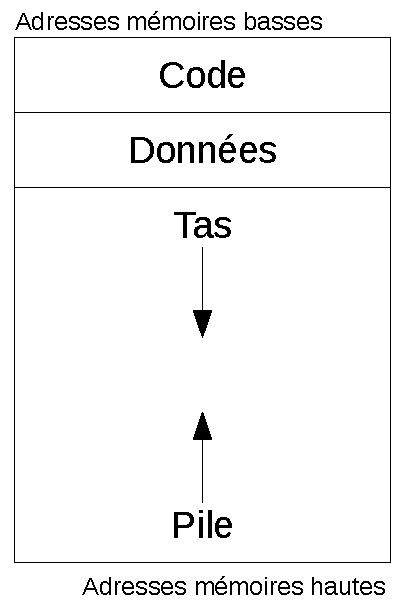
\includegraphics[width=0.3\textwidth]{supports/architecture/pile.pdf}
\todo[inline]{inverser?}
% % PSTricks TeX macro
% Title: /home/aurelien/RapportsLatex/these/supports/architecture/pile2.dia
% Creator: Dia v0.97.2
% CreationDate: Mon Jun 30 11:09:51 2014
% For: aurelien
% \usepackage{pstricks}
% The following commands are not supported in PSTricks at present
% We define them conditionally, so when they are implemented,
% this pstricks file will use them.
\ifx\setlinejoinmode\undefined
  \newcommand{\setlinejoinmode}[1]{}
\fi
\ifx\setlinecaps\undefined
  \newcommand{\setlinecaps}[1]{}
\fi
% This way define your own fonts mapping (for example with ifthen)
\ifx\setfont\undefined
  \newcommand{\setfont}[2]{}
\fi
\pspicture(-360.050000,-21.152500)(-349.950000,-3.386313)
\psscalebox{1.000000 -1.000000}{
\newrgbcolor{dialinecolor}{0.000000 0.000000 0.000000}%
\psset{linecolor=dialinecolor}
\newrgbcolor{diafillcolor}{1.000000 1.000000 1.000000}%
\psset{fillcolor=diafillcolor}
\psset{linewidth=0.100000cm}
\psset{linestyle=solid}
\psset{linestyle=solid}
\setlinejoinmode{0}
\newrgbcolor{dialinecolor}{1.000000 1.000000 1.000000}%
\psset{linecolor=dialinecolor}
\pspolygon*(-360.000000,5.000000)(-360.000000,20.000000)(-350.000000,20.000000)(-350.000000,5.000000)
\newrgbcolor{dialinecolor}{0.000000 0.000000 0.000000}%
\psset{linecolor=dialinecolor}
\pspolygon(-360.000000,5.000000)(-360.000000,20.000000)(-350.000000,20.000000)(-350.000000,5.000000)
\setfont{Helvetica}{0.800000}
\newrgbcolor{dialinecolor}{0.000000 0.000000 0.000000}%
\psset{linecolor=dialinecolor}
\rput[l](-360.000000,4.000000){\psscalebox{1 -1}{addresses mémoire basses}}
\setfont{Helvetica}{0.800000}
\newrgbcolor{dialinecolor}{0.000000 0.000000 0.000000}%
\psset{linecolor=dialinecolor}
\rput[l](-359.000000,21.000000){\psscalebox{1 -1}{addresses mémoire hautes}}
\psset{linewidth=0.100000cm}
\psset{linestyle=solid}
\psset{linestyle=solid}
\setlinejoinmode{0}
\newrgbcolor{dialinecolor}{1.000000 1.000000 1.000000}%
\psset{linecolor=dialinecolor}
\pspolygon*(-360.000000,5.000000)(-360.000000,7.000000)(-350.000000,7.000000)(-350.000000,5.000000)
\newrgbcolor{dialinecolor}{0.000000 0.000000 0.000000}%
\psset{linecolor=dialinecolor}
\pspolygon(-360.000000,5.000000)(-360.000000,7.000000)(-350.000000,7.000000)(-350.000000,5.000000)
\setfont{Helvetica}{0.800000}
\newrgbcolor{dialinecolor}{0.000000 0.000000 0.000000}%
\psset{linecolor=dialinecolor}
\rput[l](-357.000000,6.000000){\psscalebox{1 -1}{}}
\setfont{Helvetica}{0.800000}
\newrgbcolor{dialinecolor}{0.000000 0.000000 0.000000}%
\psset{linecolor=dialinecolor}
\rput(-355.000000,6.000000){\psscalebox{1 -1}{Code}}
\psset{linewidth=0.100000cm}
\psset{linestyle=solid}
\psset{linestyle=solid}
\setlinejoinmode{0}
\newrgbcolor{dialinecolor}{1.000000 1.000000 1.000000}%
\psset{linecolor=dialinecolor}
\pspolygon*(-360.000000,7.000000)(-360.000000,9.000000)(-350.000000,9.000000)(-350.000000,7.000000)
\newrgbcolor{dialinecolor}{0.000000 0.000000 0.000000}%
\psset{linecolor=dialinecolor}
\pspolygon(-360.000000,7.000000)(-360.000000,9.000000)(-350.000000,9.000000)(-350.000000,7.000000)
\setfont{Helvetica}{0.800000}
\newrgbcolor{dialinecolor}{0.000000 0.000000 0.000000}%
\psset{linecolor=dialinecolor}
\rput[l](-357.000000,8.000000){\psscalebox{1 -1}{}}
\setfont{Helvetica}{0.800000}
\newrgbcolor{dialinecolor}{0.000000 0.000000 0.000000}%
\psset{linecolor=dialinecolor}
\rput(-355.000000,8.000000){\psscalebox{1 -1}{Données}}
\setfont{Helvetica}{0.800000}
\newrgbcolor{dialinecolor}{0.000000 0.000000 0.000000}%
\psset{linecolor=dialinecolor}
\rput(-355.000000,19.221250){\psscalebox{1 -1}{Pile}}
\newrgbcolor{dialinecolor}{1.000000 1.000000 1.000000}%
\psset{linecolor=dialinecolor}
\pspolygon*(-355.505000,9.405000)(-355.505000,10.152500)(-354.495000,10.152500)(-354.495000,9.405000)
\setfont{Helvetica}{0.800000}
\newrgbcolor{dialinecolor}{0.000000 0.000000 0.000000}%
\psset{linecolor=dialinecolor}
\rput(-355.000000,10.000000){\psscalebox{1 -1}{Tas}}
\psset{linewidth=0.100000cm}
\psset{linestyle=dotted,dotsep=0.200000}
\psset{linestyle=dotted,dotsep=0.200000}
\setlinecaps{0}
\newrgbcolor{dialinecolor}{0.000000 0.000000 0.000000}%
\psset{linecolor=dialinecolor}
\psline(-355.000000,11.000000)(-355.000000,12.513197)
\psset{linestyle=solid}
\setlinejoinmode{0}
\setlinecaps{0}
\newrgbcolor{dialinecolor}{0.000000 0.000000 0.000000}%
\psset{linecolor=dialinecolor}
\pspolygon*(-355.000000,12.888197)(-355.250000,12.388197)(-355.000000,12.513197)(-354.750000,12.388197)
\newrgbcolor{dialinecolor}{0.000000 0.000000 0.000000}%
\psset{linecolor=dialinecolor}
\pspolygon(-355.000000,12.888197)(-355.250000,12.388197)(-355.000000,12.513197)(-354.750000,12.388197)
\psset{linewidth=0.100000cm}
\psset{linestyle=dotted,dotsep=0.200000}
\psset{linestyle=dotted,dotsep=0.200000}
\setlinecaps{0}
\newrgbcolor{dialinecolor}{0.000000 0.000000 0.000000}%
\psset{linecolor=dialinecolor}
\psline(-355.000000,18.000000)(-355.000000,16.486803)
\psset{linestyle=solid}
\setlinejoinmode{0}
\setlinecaps{0}
\newrgbcolor{dialinecolor}{0.000000 0.000000 0.000000}%
\psset{linecolor=dialinecolor}
\pspolygon*(-355.000000,16.111803)(-354.750000,16.611803)(-355.000000,16.486803)(-355.250000,16.611803)
\newrgbcolor{dialinecolor}{0.000000 0.000000 0.000000}%
\psset{linecolor=dialinecolor}
\pspolygon(-355.000000,16.111803)(-354.750000,16.611803)(-355.000000,16.486803)(-355.250000,16.611803)
}\endpspicture
% \missingfigure{!}
\caption{Organisation de la mémoire d'un processus}
\label{fig:mem_process}
\end{center}
\end{figure}

\paragraph{Jeu d'instructions.}
Les processeurs Intel \xq\ utilisent un jeu d'instruction complexe (CISC). La représentation d'une instruction en une suite d'octets inclut principalement un code d'opération et ses arguments. Des informations supplémentaire peuvent être codées dans l'instruction, comme des préfixes. Le format des instructions détaillé est donné figure \ref{fig:format_insts_x86}.
L'instruction \texttt{mov ecx, 0x080490a4} de la figure \ref{fig:text_helloworld}, codée sur \texttt{b9 a4 90 04 08} est composée de l'opcode \texttt{b8+r} indiquant une opération de copie d'une valeur immédiate vers un registre. Ici r est égal à 1, ce qui indique que le registre concerné est ecx. La valeur à copier vers le registre est 0x080490a4 soient les octets \texttt{a4 90 04 08} codés en petit-boutistes (\emph{little endianness}), c'est à dire que les mots de poids faibles sont écrits en premiers, à l'inverse de l'écriture usuelle.
Il s'agit d'une assignation immédiate et la valeur à copier vers \texttt{ecx} est la valeur immédiate.
Le décalage permet de modifier une instruction d'adressage indirect comme \texttt{mov ecx, [eax]}, écrivant le contenu en mémoire à l'adresse \texttt{eax} dans le registre \texttt{ecx} en \texttt{mov ebx, [eax+d]} où \texttt{d} est le décalage.
Enfin les préfixes permettent par exemple de répéter plusieurs fois l'instruction jusqu'à ce qu'une condition sur un registre soit remplie.

\begin{figure}
\begin{center} 
\begin{tabular}{l|l|l|l|l|l|}
\cline{2-6}
% Prefixe & Opcode & Modificateur & SIB & Déplacement d'octet & Adressage\\
% 1 à 4 & 1 à 3 & 0 ou 1 & 0 ou 1 & 0 à 4 & 0 à 4\\
& Préfixe & Opcode & Modificateur & Décalage & Valeur immédiate \\
& 1 à 4 & 1 à 3 & 0 à 2 & 0 à 4 & 0 à 4\\
\cline{2-6}
\multicolumn{1}{l}{Exemples :} & \multicolumn{5}{l}{}\\
\hline
\multicolumn{1}{|l|}{mov ecx, 0x080490a4} & & b9 & & & a4 90 04 08 \\
\multicolumn{1}{|l|}{add eax, 2} & & 83 & c0 & & 02 \\
\hline
\end{tabular}
\end{center} 
\caption{Format d'une instruction \xq\ et taille des opérandes en octets}
\label{fig:format_insts_x86}
\end{figure}

\paragraph{Intuition de sémantique.}
% ~\\
% \todo[inline]{assignations (déplacement en mémoire)\\
% opérations arithmétique\\
% controle de flot inconditionnel\\
% conditionnel}
% 
% \todo[inline]{effets de bords\\
% explicites\\
% implicites}

Bien que la documentation exhaustive d'Intel pour les processeurs \xq\ et \xs\ \cite{intel_vol2} détaille plusieurs centaines d'instructions, elles peuvent être regroupées en 3 classes informelles.
Prenons l'instruction \texttt{mov} : elle sert à copier des informations depuis une zone (mémoire ou registre) vers une autre zone.
Ainsi \texttt{mov eax, [ebx+10]} copie la valeur à l'adresse \texttt{ebx+10} dans le registre \eax. 
Cette instruction est déclinée en plusieurs dizaines de variantes selon la taille et le type des opérandes copiés.

Une seconde catégorie d'instructions permet de gérer les opérations arithmétiques sur les octets en mémoire et dans les registres.
Une instructions comme \texttt{add eax, ebx} ajoute la valeur de \ebx\ à celle de \eax\ et stocke le résultat de l'opération dans \eax.
Ce type d'opération combine en fait une opération arithmétique et une assignation. 
On peut y inclure l'instruction \cmp\ qui compare deux valeurs et met à jour les drapeaux de tests. 
Ces drapeaux indiquent entre autres le signe du résultat d'une opération ainsi que si elle a provoqué un débordement d'entier (dans le cas où le résultat est trop grand pour être stocké sur un entier).
En fait les instructions arithmétiques comme \add\ provoquent aussi une mise à jour de ces drapeaux : il s'agit d'une assignation implicite.\jym{sens ? expliquer ce qu'on veut dire par explicite/implicite?}

Les instructions précédemment décrites sont séquentielles et ne modifient pas l'ordre d'exécution d'une instruction. 
Après l'exécution d'une instruction de type \mov\ à l'adresse $a$ codée sur $n$ octets, l'instruction située à l'adresse $a+n$.
Le dernier type d'instruction modifie le flot de contrôle du programme et effectuent des sauts à des adresses spécifiées dans le programme.
Ces sauts peuvent être inconditionnels comme un \texttt{jmp 8048085} qui provoque un saut à l'adresse \texttt{8048085} ou le saut dynamique \texttt{jmp eax} dont l'adresse cible du saut est la valeur de \eax.
Les sauts peuvent aussi être conditionnels : \texttt{je +10}, à l'adresse $a$ et de taille $n$, sera suivie de l'instruction à l'adresse $a+10$ si le registre ZF vaut 1 (en cas d'égalité) et de l'instruction à l'adresse $a+n$ dans le cas contraire.

\ijym{parler du multi-threading, de cores et de l'accès mémoire en cas de multi-threading}


\section{Analyse de code binaire}
\itodo{changer en : difficultés de l'analyse}
\itodo{perte d'informations de haut niveau}
Le désassemblage est l'opération inverse de l'assemblage : il consiste à récupérer le code assembleur source du binaire.
Cette tâche semble particulièrement simple puisque l'assemblage consiste simplement à trouver les octets correspondants à chaque instruction à l'aide de la documentation officielle du processeur puis à mettre en forme le fichier binaire en remplissant correctement ses entêtes et ses sections.
Pourtant on a vu que, dans le modèle de Harvard modifié, les données et le code peuvent être mêlés. 
En particulier les parties de données (comme la section \pdata) peuvent être exécutées. 
De même les sections de code peuvent contenir des informations destinées à être simplement lues ou modifiées mais jamais exécutées.
La difficulté du désassemblage consiste donc à séparer les parties potentiellement exécutables des données.

Ainsi un désassemblage à priori cohérent de \helloworld\ consisterait à considérer les deux sections comme contenant du code potentiellement exécutable. Ce désassemblage sera composé de la section \ptext\ déjà désassemblé Figure \ref{fig:text_helloworld} et la section \pdata\ donnée Figure \ref{fig:data_exec_helloworld}.
Ce désassemblage n'est pas correct et on peut le prédire. 
On connaît le point d'entrée du binaire, qui est l'adresse \texttt{8048080} dans la section \ptext.
Les instructions exécutées dans la section \ptext\ à la suite du point d'entrée sont séquentielles et ne peuvent détourner l'exécution vers la section \pdata. 
Le code désassemblé dans cette section n'est donc pas atteignable. Dans ce cas on sait alors que la section \pdata\ ne contient pas de code et ne doit pas être désassemblée.

\begin{figure}
\begin{center}
\begin{tabular}{|c|c|l|l|}
\hline
Emplacement & Adresses de chargement & Octets & Instruction\\ 
dans le fichier & &  & \\ 
\hline
94 & 80490a4 & 48    & dec    eax			\\
95 & 80490a5 & 65    & gs				\\
96 & 80490a6 & 6c    & ins    BYTE PTR es:[edi],dx	\\
97 & 80490a7 & 6c    & ins    BYTE PTR es:[edi],dx	\\
98 & 80490a8 & 6f    & outs   dx,DWORD PTR ds:[esi]	\\
99 & 80490a9 & 2c 20 & sub    al,0x20			\\
9b & 80490ab & 77 6f & ja     0x804911c			\\
9d & 80490ad & 72 6c & jb     0x804911b			\\
9f & 80490af & 64    & fs				\\
a0 & 80490b0 & 0a    & .byte 0xa			\\
\hline
\end{tabular}
\end{center}
\caption{Section \pdata\ de \helloworld\ désassemblée comme du code}
\label{fig:data_exec_helloworld}
\end{figure}

% \paragraph{Utilisation de sauts dynamiques.}
En pratique un programme est constitué d'un grand nombre d'instructions de saut et notamment de sauts dynamiques de type \texttt{jmp eax}.
Ce type d'instructions posent un souci lors de l'analyse : sans connaître précisément la ou les valeurs potentielles d'\eax, impossible de prédire la cible du saut et donc de savoir le code potentiellement exécuté à la suite de cette instruction.
Dans l'exemple du \helloworld, si une telle instruction est présente dans la section \ptext, il devient difficile d'exclure l'exécution possible de code dans la section \pdata.

\subsection{Reconstruction du graphe de flot de contrôle (GFC).}
Nous avons vu jusqu'ici une réprésentation des programmes assembleur et binaires sous forme de code linéaire mais il est plus aisé de visualiser les programmes à l'aide d'un graphe de flot de contrôle (GFC).
Ce graphe représente les instructions sous forme de sommets et les sauts du flot de contrôle d'une instruction à une autre sous forme d'arcs.
Prenons le programme assembleur donné en figure \ref{fig:asm_eax_code}. Il ne fait que modifier le registre \eax, effectue des sauts selon la valeur d'\eax\ et se termine avec une valeur pour \eax\ à 1 ou 2. L'instruction \texttt{mov eax, 3} n'est pas atteignable puisqu'elle suit un saut inconditionnel et qu'aucune autre instruction ne provoque un saut vers elle.
Ainsi le graphe de flot de contrôle de ce programme est celui donné en figure \ref{fig:asm_eax_cfg}.

Le sommet coloré en orange est le point d'entrée du programme. Dans le cas où le flot de contrôle peut passer de l'instruction $a$ à l'instruction $b$, l'arc entre $a$ et $b$ est en noir si $b$ suit $a$ en mémoire et en rouge sinon, c'est à dire dans le cas où il s'agit d'un saut.

Un graphe de flot idéal inclut exactement l'ensemble des instructions atteignables dans le programme et un arc ne relie deux instructions que s'il existe au moins une exécution du programme dans laquelle les deux instructions sont exécutées consécutivement.
\\

\begin{figure}
\begin{center}
\subfigure[Code assembleur]{
\begin{tabular}[b]{|l|l|l|}
\hline
Adresse & Octets & Instruction\\ 
\hline
 8048067  &  b8 00 00 00 00         &  mov    eax,0x0 \\
 804806c  &  eb 05                  &  jmp    0x8048073 \\
 804806e  &  b8 03 00 00 00         &  mov    eax,0x3 \\
 8048073  &  83 f8 00               &  cmp    eax,0x0 \\
 8048076  &  74 06                  &  je     0x804807e \\
 8048078  &  b8 01 00 00 00         &  mov    eax,0x1 \\
 804807d  &  c3                     &  ret     \\
 804807e  &  b8 02 00 00 00         &  mov    eax,0x2 \\
 8048083  &  c3                     &  ret     \\
\hline
\end{tabular}
\label{fig:asm_eax_code}
}
\subfigure[Graphe de flot de contrôle]{
% 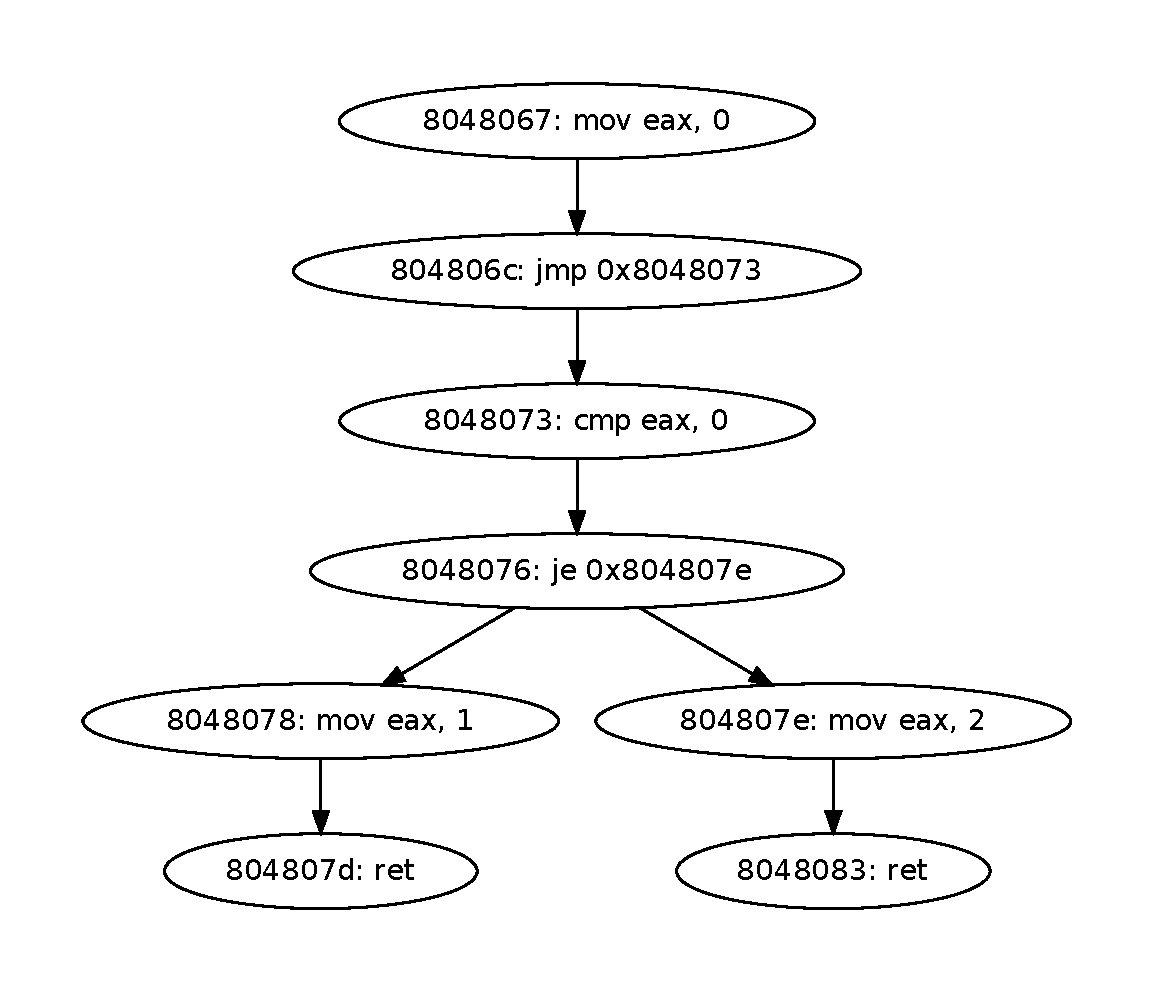
\includegraphics[width=0.6\textwidth]{supports/eax-cfg/eax.pdf}

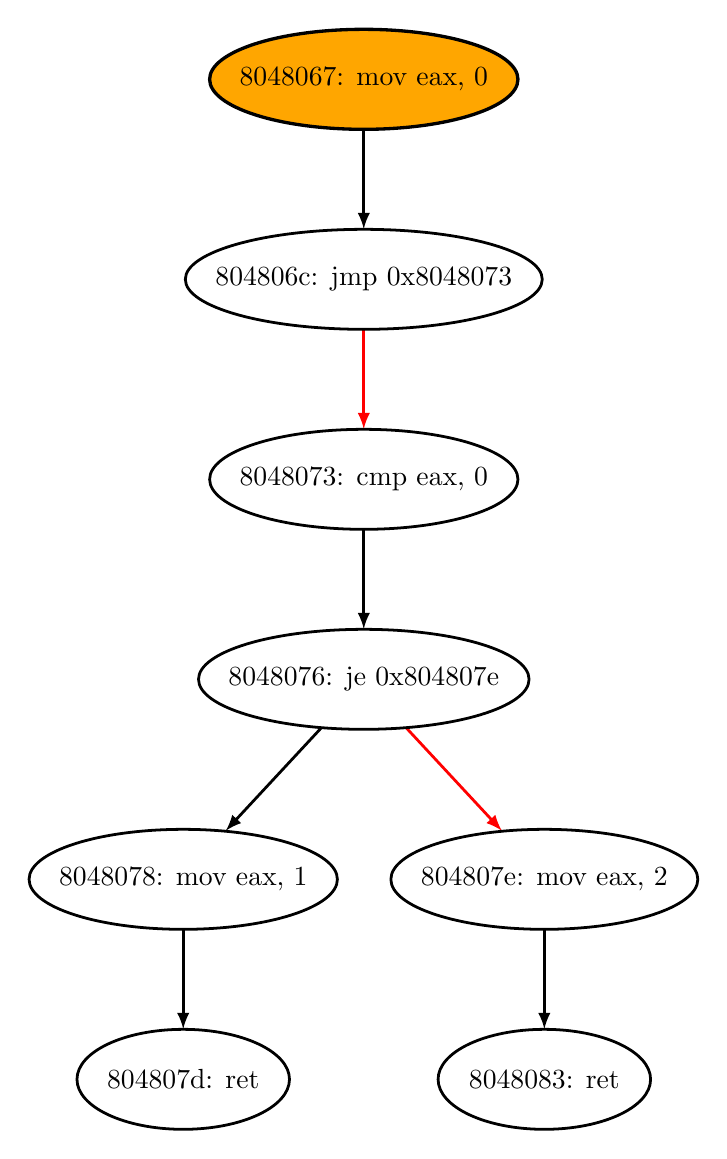
\begin{tikzpicture}[>=latex,line join=bevel,]
  \pgfsetlinewidth{1bp}
%%
\pgfsetcolor{black}
  % Edge: 5 -> 6
  \draw [->] (105.6bp,144.41bp) .. controls (97.42bp,135.61bp) and (87.226bp,124.63bp)  .. (71.294bp,107.47bp);
  % Edge: 5 -> 8
  \pgfsetcolor{red}
  \draw [->] (136.4bp,144.41bp) .. controls (144.58bp,135.61bp) and (154.77bp,124.63bp)  .. (170.71bp,107.47bp);
  % Edge: 6 -> 7
  \pgfsetcolor{black}
  \draw [->] (56.0bp,71.697bp) .. controls (56.0bp,63.983bp) and (56.0bp,54.712bp)  .. (56.0bp,36.104bp);
  % Edge: 4 -> 5
  \draw [->] (121.0bp,215.7bp) .. controls (121.0bp,207.98bp) and (121.0bp,198.71bp)  .. (121.0bp,180.1bp);
  % Edge: 1 -> 2
  \draw [->] (121.0bp,359.7bp) .. controls (121.0bp,351.98bp) and (121.0bp,342.71bp)  .. (121.0bp,324.1bp);
  % Edge: 8 -> 9
  \draw [->] (186.0bp,71.697bp) .. controls (186.0bp,63.983bp) and (186.0bp,54.712bp)  .. (186.0bp,36.104bp);
  % Edge: 2 -> 4
  \pgfsetcolor{red}
  \draw [->] (121.0bp,287.7bp) .. controls (121.0bp,279.98bp) and (121.0bp,270.71bp)  .. (121.0bp,252.1bp);
  % Node: 1
\begin{scope}
  \definecolor{strokecol}{rgb}{0.0,0.0,0.0};
  \pgfsetstrokecolor{strokecol}
  \definecolor{fillcol}{rgb}{1.0,0.65,0.0};
  \pgfsetfillcolor{fillcol}
  \filldraw [opacity=1] [very thick] (121.0bp,378.0bp) ellipse (55.5bp and 18.0bp);
  \draw (121.0bp,378.0bp) node {8048067: mov eax, 0};
\end{scope}
  % Node: 2
\begin{scope}
  \definecolor{strokecol}{rgb}{0.0,0.0,0.0};
  \pgfsetstrokecolor{strokecol}
  \draw (121.0bp,306.0bp) ellipse (64.25bp and 18.0bp);
  \draw (121.0bp,306.0bp) node {804806c: jmp 0x8048073};
\end{scope}
  % Node: 5
\begin{scope}
  \definecolor{strokecol}{rgb}{0.0,0.0,0.0};
  \pgfsetstrokecolor{strokecol}
  \draw (121.0bp,162.0bp) ellipse (59.5bp and 18.0bp);
  \draw (121.0bp,162.0bp) node {8048076: je 0x804807e};
\end{scope}
  % Node: 4
\begin{scope}
  \definecolor{strokecol}{rgb}{0.0,0.0,0.0};
  \pgfsetstrokecolor{strokecol}
  \draw (121.0bp,234.0bp) ellipse (55.5bp and 18.0bp);
  \draw (121.0bp,234.0bp) node {8048073: cmp eax, 0};
\end{scope}
  % Node: 7
\begin{scope}
  \definecolor{strokecol}{rgb}{0.0,0.0,0.0};
  \pgfsetstrokecolor{strokecol}
  \draw (56.0bp,18.0bp) ellipse (38.25bp and 18.0bp);
  \draw (56.0bp,18.0bp) node {804807d: ret};
\end{scope}
  % Node: 6
\begin{scope}
  \definecolor{strokecol}{rgb}{0.0,0.0,0.0};
  \pgfsetstrokecolor{strokecol}
  \draw (56.0bp,90.0bp) ellipse (55.5bp and 18.0bp);
  \draw (56.0bp,90.0bp) node {8048078: mov eax, 1};
\end{scope}
  % Node: 9
\begin{scope}
  \definecolor{strokecol}{rgb}{0.0,0.0,0.0};
  \pgfsetstrokecolor{strokecol}
  \draw (186.0bp,18.0bp) ellipse (38.25bp and 18.0bp);
  \draw (186.0bp,18.0bp) node {8048083: ret};
\end{scope}
  % Node: 8
\begin{scope}
  \definecolor{strokecol}{rgb}{0.0,0.0,0.0};
  \pgfsetstrokecolor{strokecol}
  \draw (186.0bp,90.0bp) ellipse (55.25bp and 18.0bp);
  \draw (186.0bp,90.0bp) node {804807e: mov eax, 2};
\end{scope}
%
\end{tikzpicture}


\label{fig:asm_eax_cfg}
}
\end{center}
\caption{Représentation d'une fonction assembleur modifiant \eax}
\label{fig:asm_eax}
\end{figure}


\subsection{Parcours linéaire}
Un désassemblage suivant un parcours linéaire désassemble, pour chaque section, la première instruction à l'adresse $a$ puis l'instruction à l'adresse $a+k$ où $k$ est le nombre d'octets sur lesquels l'instruction est codée.
Ainsi pour une suite d'instructions séquentielles cette méthode suit le flot de contrôle mais si une instruction de type \jmp\ est rencontrée, le désassemblage s'intéressera à l'instruction qui suit en mémoire et non celle qui sera logiquement exécutée ensuite.
La figure \ref{fig:asm_eax_code} donne un exemple de désassemblage linéaire d'une fonction assembleur.
L'avantage de cette technique réside dans sa simplicité et le fait qu'elle couvre l'ensemble de la mémoire.
Pourtant, ne cherchant pas à suivre le flot de contrôle, elle ne permet pas de séparer le code exécutable des données et désassemble des instructions qui ne sont pas atteignables comme l'instruction \mov\ à l'adresse $804806e$ de la figure \ref{fig:asm_eax}.
C'est l'approche utilisée par le désassembleur standard du projet GNU, objdump \cite{objdump}.
\todo[inline]{radare?}

\subsection{Parcours récursif}
À l'inverse du parcours linéaire, le parcours récursif suit le flot de contrôle et désassemble les instructions qui se suivent logiquement en partant du point d'entrée du programme. Le graphe de flot de contrôle peut être déduit du parcours récursif : la figure \ref{fig:asm_eax_cfg} donne celui de l'exemple précédent.
Une telle approche est utilisée par le désassembleur commercial IDA \cite{IDA}.
L'avantage de cette technique est qu'elle ne désassemble que des instructions dont on peut raisonnablement penser qu'elles sont atteignables.

Cependant certains chemins ne sont pas atteignables en raison de variables définies. 
L'instruction à l'adresse \texttt{8048076} provoque un saut vers l'adresse \texttt{804807e} si la comparaison effectuée à l'instruction précédente est vraie, c'est à dire si $\eax=0$, et saute vers l'adresse \texttt{8048078} dans le cas contraire.
Or la première instruction de la fonction donne à \eax\ la valeur 0. Dans tous les cas le saut se produira donc vers l'adresse \texttt{804807e} et l'autre branche n'est pas atteignable.

D'autre part si des sauts dynamiques sont utilisés comme avec l'instruction \texttt{jmp eax}, le parcours récursif s'arrête alors qu'il est clair que d'autres instructions seront exécutées.
\jym{déterminer eax peut être indécidable // le pb vient des embranchements et des prédicats opaques ?}




% \todo[inline]{
% Réorganisation du code \\
% Aplatissement de CFG \\
% }

% \section{Difficulté calculatoire de l'analyse de binaire}
% \subsection{Désassemblage}
% \subsection{Décompilation}